\section{Задание 2: Решить задачи Коши}
    \subsection{Постановка задачи}
        Для заданных уравнений указать тип в простой форме. Найти общее решение. Найти частное решение, удовлетворяющее заданным условиям. Построить график решения:

        \begin{enumerate}
            \item \( x^2 y'' - 3xy' = \frac{6y^2}{x^2} - 4y; y(1) = 1, y'(1) = 4; \)
            \item \( y'y'' - \sqrt{1+y'^2} = 0; y(0) = y'(0) = 0. \)
        \end{enumerate}

    
    \subsection{Решение}
        \begin{enumerate}
            \item \( \begin{cases}
                x^2 y'' - 3xy' = \frac{6y^2}{x^2} - 4y, \\
                y(1) = 1, y'(1) = 4;
            \end{cases} \) \label{eq1}
            
                \textit{Тип уравнения:}
                    Обобщённое однородное уравнение;
                
                \textit{Общее решение:}
                    \( \left( \frac{y'}{x} - 2 \frac{y}{x^2} \right)^2 = 4 \frac{y^3}{x^6} + C_1 \);

                
                \textit{Частное решение:}
                    \( y = \frac{x^2}{\left( 1 - \ln x \right)^2} \)

                \begin{figure}[H]
                    \centering
                    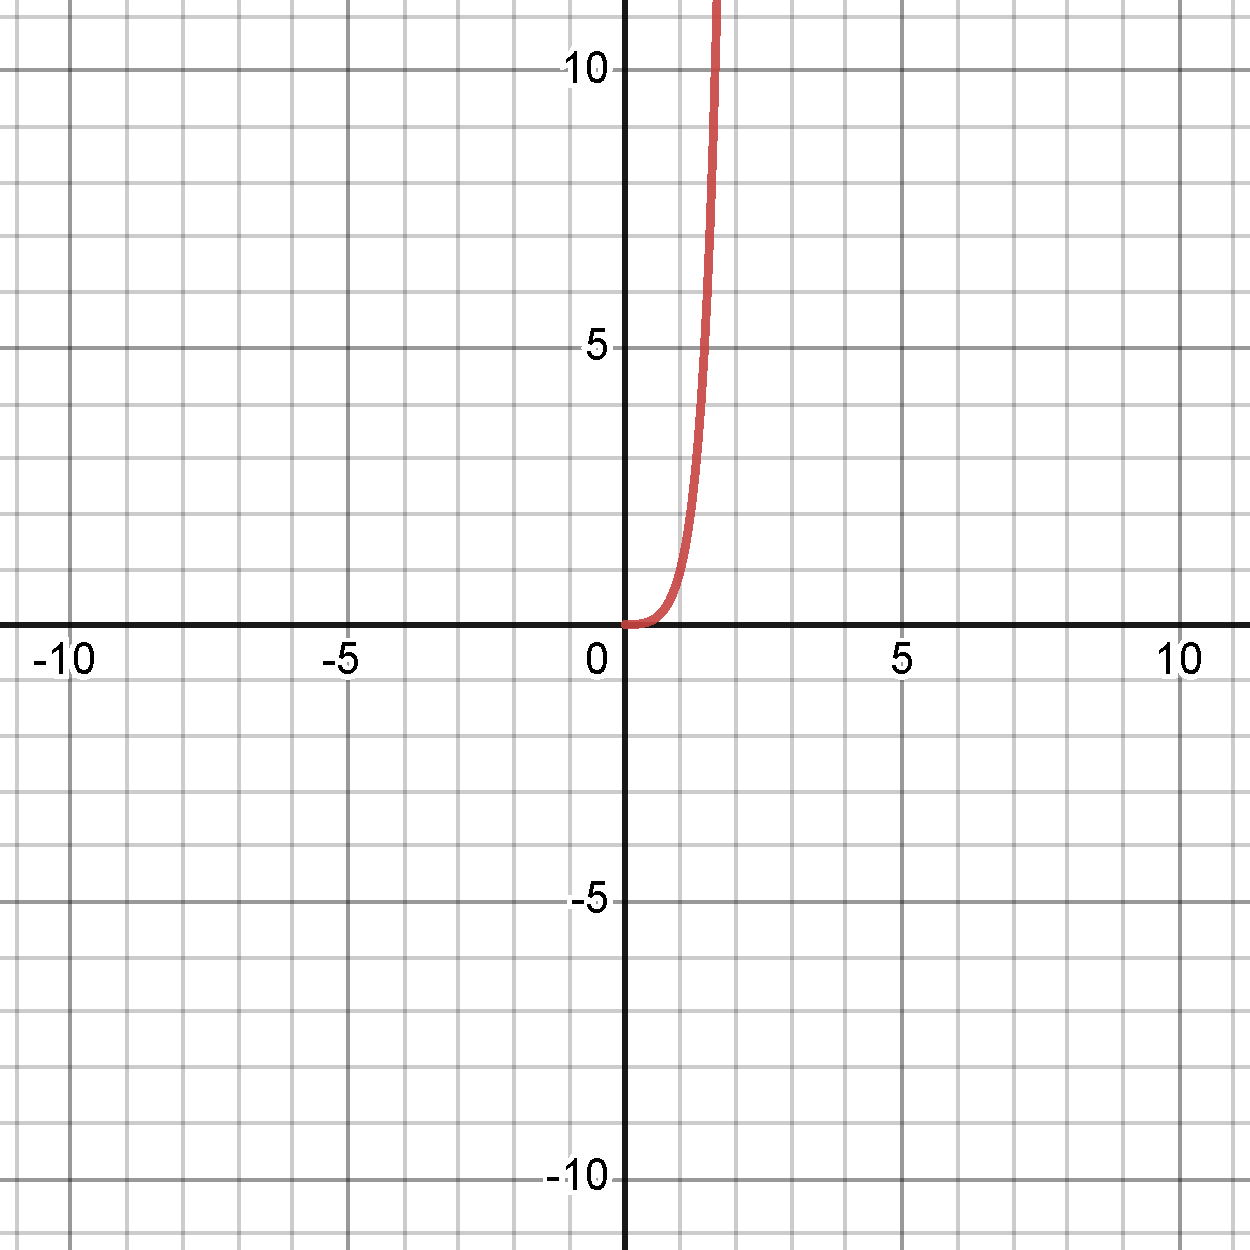
\includegraphics[width=7cm]{pictures/task2_1.pdf}
                    \caption{График решения уравнения (\ref{eq1})}
                \end{figure}
            
            \pagebreak
            
            \item \( \begin{cases}
                y'y'' - \sqrt{1+y'^2} = 0, \\
                y(0) = y'(0) = 0;
            \end{cases} \) \label{eq2}
            
                \textit{Тип уравнения:}
                    Вполне интегрируемое уравнение.
                
                \textit{Общее решение:}
                    \[ 
                        2y = \pm\left( (x + C_1) \sqrt{(x+C_1)^2 - 1} - \ln \left( \sqrt{(x+C_1)^2 - 1} + x + C_1 \right) \right) + C_2 
                    \]
                
                \textit{Частное решение:}
                    \( 
                        2y = \pm\left((x + 1) \sqrt{x^2 + 2x} - \ln \left( \sqrt{x^2 + 2x} + x + 1 \right)\right);
                    \)

                \begin{figure}[H]
                    \centering
                    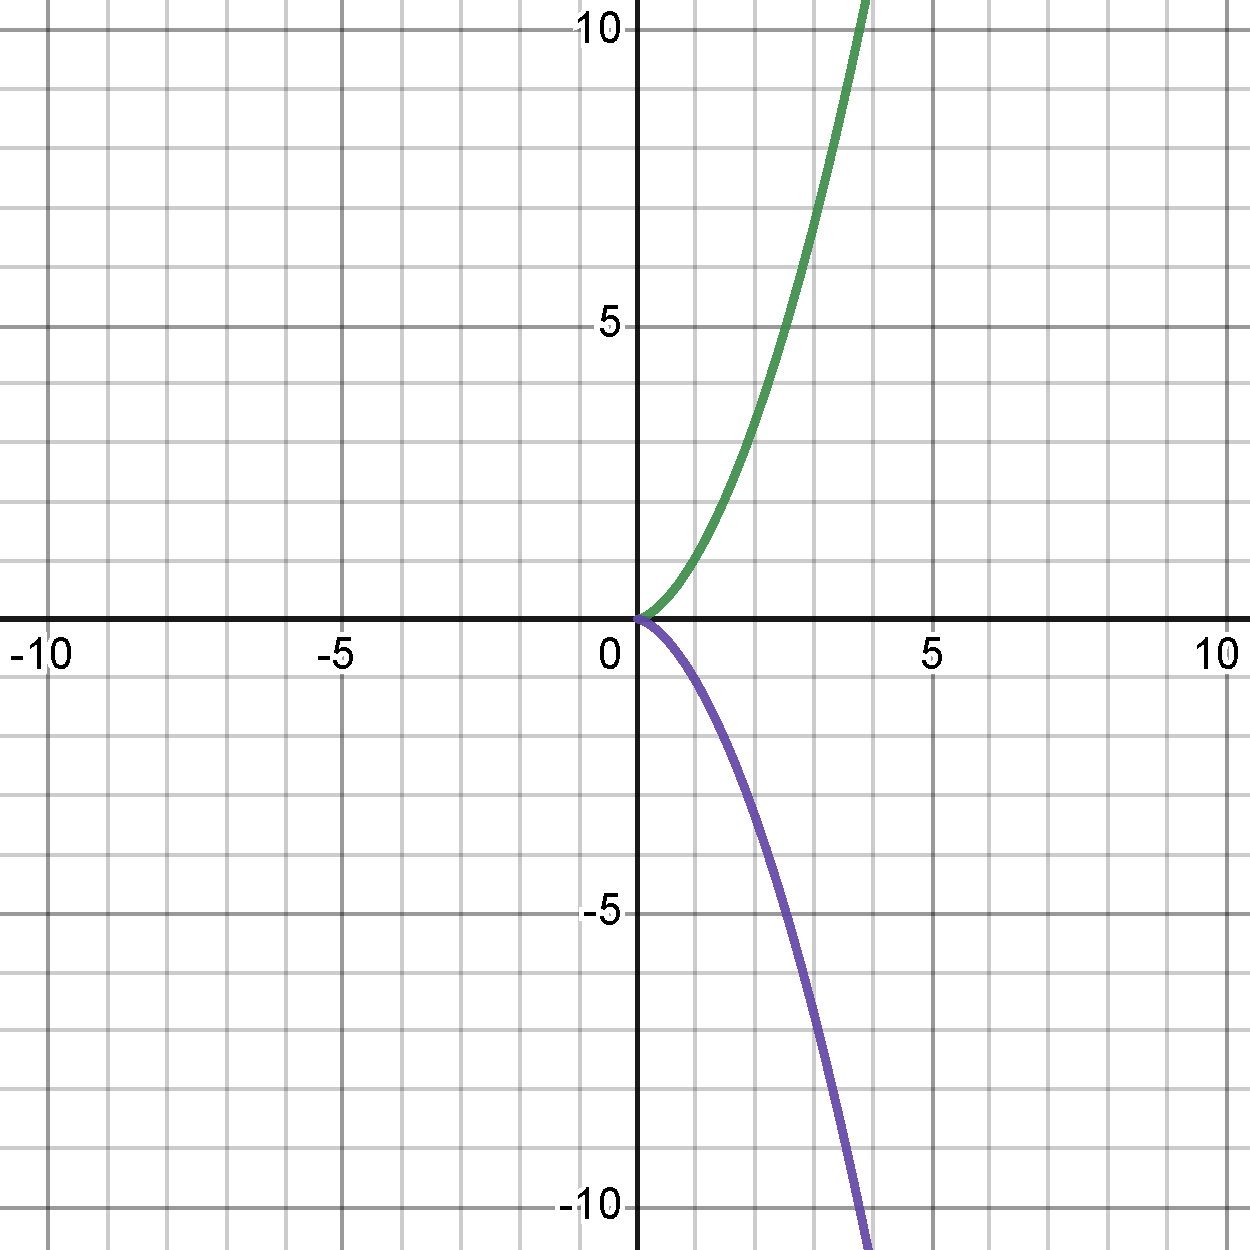
\includegraphics[width=7cm]{pictures/task2_2.pdf}
                    \caption{График решения уравнения (\ref{eq2})}
                \end{figure}

        \end{enumerate}